\section{Taxonomy of Separation and Perception}

With the previous work of creating effective and efficient algorithms for DR a lack of guidance for the user of certain models or algorithms has occurred~\cite{sedlmair2012taxonomy,friendly2005early}. The question how and to what extend a user can be supported and shown what DR and VE techniques to use is a non-trivial task~\cite{sedlmair2012taxonomy}.

The DimStiller system uses a workflow structure to guide users through the process of choosing DE and VE techniques~\cite{ingram2010dimstiller}, but automatic algorithms to provide such guidance have not yet emerged. To service this goal Sedlmair et al. used visual cluster separation measures~\cite{sips2009selecting, tatu2009combining}, originally developed for selecting good views within \underline{s}catter\underline{pl}ot \underline{m}atricies (SPLOM), to provide guidance for DR and VE technique choices. Two particular measures have been identified as the most effective: the \textbf{centroid} and the \textbf{grid} measure~\cite{tatu2010visual}. These names where chosen by Sedlmair et al. for readability and have been named other by different researchers~\cite{sedlmair2012taxonomy}.

They further showed that these measures fail to produce reliable results, meaning it resulted in a mismatch between the algorithms results and the quality judgement made by a person~\cite{sedlmair2012taxonomy}. The two cases of false positives and false negatives occurred; either the algorithm showed that a distinct measure was sufficient for a convincing separation to happen, but the human judged the visual separation as poor, or the algorithm failed to provide such separation but humans were indeed able to distinguish clusters in scatterplots.

These measures can be used in multiclass density maps to select the tiling, the separation of data into tiles, and thus enhance the visual impression.

% \info{two human investigators evaluated separation factors}

\subsection{Visual Cluster Separation Factors}

The general idea behind all existing separation measures is to evaluate how "pure" the neighborhoods of a scatterplot's data points are. If neighborhoods include points from many different classes they are intermixed, if only one class then they are pure~\cite{aupetit2016sepme}.
The general concept to differentiate between clusters remain generally the same and differ only based on the definitions of a neighborhood around points. Based on the work of Aupetit et al. the two definitions chosen are~\cite{aupetit2016sepme}:

\begin{itemize}[leftmargin=*]
	\setlength\itemsep{0.1em}
	\item measures with \textit{hard-neighborhoods} looks at a specific subset of the data points close to the one under focus
	\item measures with a \textit{soft-neighborhood} use the weighting of all the data points with respect to a focus point.
\end{itemize}

Local class-purity values are averaged over all possible focus points. This gives a higher purity when the local neighborhood class-purity is high for a large set of focal points, resulting in a good separation of clusters.

The separation of classes in scatterplots and density maps is dependent on different features of the plot. Participants of a study conducted by van Onzenoodt et al. indicate that spread and density of scatterplots have influence on the perception of clusters~\cite{van2017evaluating}.
When viewing scatterplots or density maps these factors are not calculated based on the mentioned approaches but rather the visual perception of clusters. This is based on each persons subjective perception of correlation and clusters~\cite{rensink2010perception, beyth1982perception, tatu2010visual}. This process can be supported by design. When the designers of maps construct the plot numerous approaches can be taken to enhance the desired effects. Some points of reference, amongst others, include count, size or density as can be seen in Figure~\ref{fig:separation_factors}. Design choices result in the improved comprehension of scatterplots and density maps.

Because multiclass scatterplots and density maps have a class property with items that need to be distinguishable, Figure~\ref{fig:separation_factors} focuses on the factors that enhance this nature and neglects within-class factors. Between-Class factors encapsulate the variance and combination of Within-Class factors across multiple classes. These factors are not described here because of the multiclass viewpoint in multiclass density maps. In the Scale section of Figure~\ref{fig:separation_factors}, the \textit{count} factor is the ratio between the number of classes and the number of points of the dataset. Sedlmair et al. found that fewer classes and many points was easier to perceive than the case of many classes, few points~\cite{sedlmair2012taxonomy}. \\
The first factor \textit{variance of density} is the mutual product of \textit{variance of size} and \textit{variance of count}. In plots where a big class is overlapping a smaller class the latter one might be identified more easily because of the law of proximity from common Gestalt psychology~\cite{kim2008object}. This is a result of a dense class being easily identifiable over sparse data.\\
The variance of shape factor ranges from similar shapes for all clusters to very different shapes across each cluster. When applied to density maps one shape might be applied to one class of data points. This will result in a mixture of shapes across the plot where a fine distinction needs to be done for the shape to be easily distinguishable to all other shapes used in the plot~\cite{borgo2013glyph, demiralp2014learning}.\\
% \textcolor{red}{\lipsum[1]}\improvement{Wtire about Demiralp et al.}
The inner-outer position in the position category describes a positional relationship between classes where a inner class can be surrounded by outer classes. Sedlmair et al. distinguish between \textit{existent} and \textit{non-existent} relations~\cite{sedlmair2012taxonomy}. They further showed that inner classes were more difficult to identify, especially those in the synthetic-gaussian data family. This shows that density maps must countermeasure this behavior with correct design adaptations.

The overarching factor is class separation. In data plots with two well separated, round, and contiguous clusters, data separation can be strongly influenced by nearly every other factor~\cite{sedlmair2012taxonomy}. For density maps the separation of classes could be the most viable factor to countermeasure the effects mentioned, mixing and masking, where data gets overlaid by other properties. In these kinds of maps it might not always be possible to apply sufficient class separation without sophisticating the two dimensional properties so designers must reside to different measures like axis scaling or using endorsed color schemes.

All of these factors can more or less be applied to multiclass density maps and the Class Buffer model, where the most significant difference is the work done before plotting the data.

\begin{figure}
	\centering
	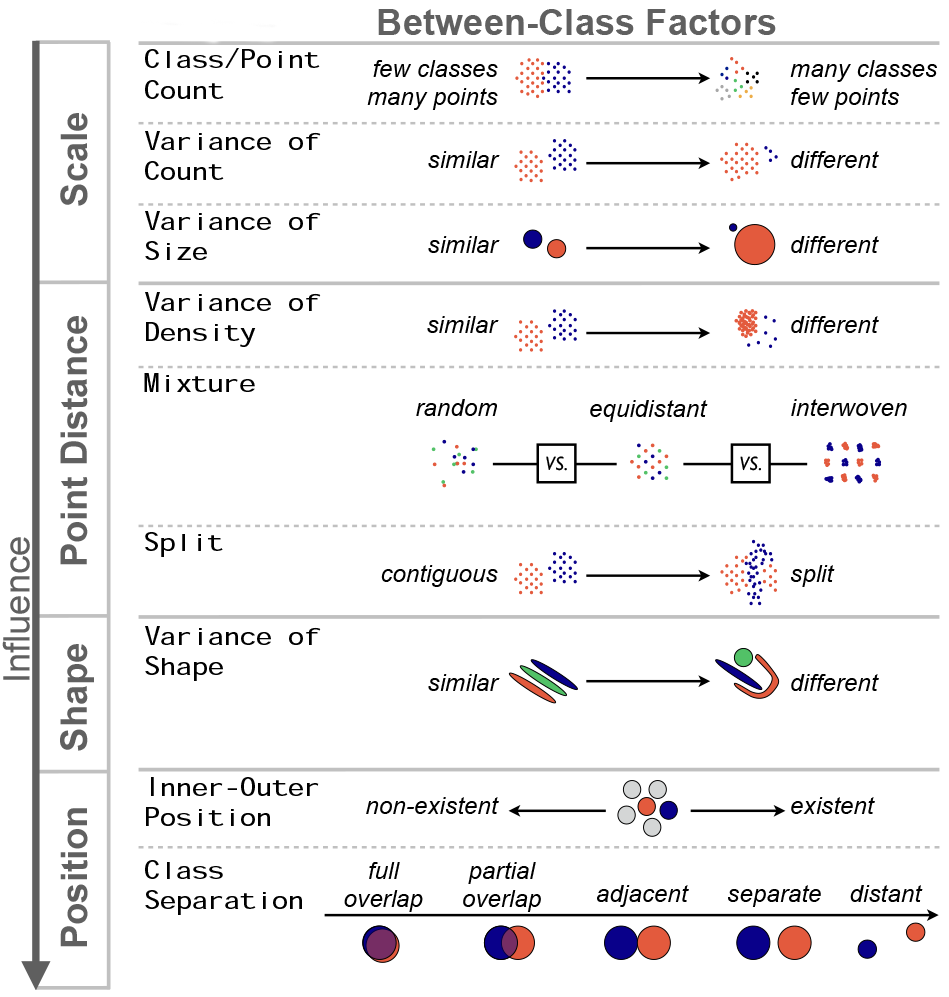
\includegraphics[width=\columnwidth]{./figures/separation}
	\caption[Separation Factors]{A taxonomy of data characteristics with respect to class separation in scatterplots. Some factors are organized as axes (arrows) while others are binned. Factors at the top can strongly influence factors below them. Class Separation is therefore dependent on all other factors.}~\label{fig:separation_factors}
\end{figure}

\subsection{Perception of Classes an Outliers}

How well different points of data are perceived in the scatterplot and density maps is a relevant task for any group of data, or even individual points. Micallef et al. focused on classes and outliers when investigating the perception within plots~\cite{micallef2017towards}.
They employ structural similarity~\cite{wang2004image} to measure the perceivability of a group of points. Structural similarity is a highly reliable image quality assessment model often applied to measure the similarity between two images~\cite{micallef2017towards}. Details on this algorithm can be taken from Wang et al.~\cite{wang2004image}.
The mean structural similarity as implemented in scikit-image~\cite{van2014scikit} can be used an applied to parts of the data with non-zero opacity. In the case of two scatterplots a and b the mean structural similarity $SSIM(a;b)$ returns values between 0 and 1, where 1 denotes that images a and b are identical.
In a case where the data of two scatterplots are almost identical but one map has a group of data points that the other one does not have, structural similarity can be taken to measure the perceived similarity between these two plots. If they are rather similar, the group of points is difficult to perceive. If the two scatterplots are rather different, then the group of points is easy to perceive~\cite{micallef2017towards}.

Overall, once users are familiar with the visualized data, they find it less difficult to perceive clusters~\cite{van2017evaluating}. Users could thus be trained to perceive classes more easily when applying similar design patterns to plots. Further, when users view multiple scatterplots or density maps they might get better at understanding these.
% \cite{aupetit2016sepme,sedlmair2012taxonomy, rensink2010perception,micallef2017towards}
